\section{Exercise 3 - Combining \texttt{MPI} Processes}

With the goal of saving slightly on communication rounds by combining a pipelined reduction and a 
pipelined broadcast more tightly to keep the processes “more busy”, we end up with the function implementation 
of \texttt{MY\_Allreduce\_P()}. This implementation is completely based on the pipelined tree 
implementation for exercise 5 (see chapter \ref{chapter_5_reference}). For better understanding, refer to exercise 5 first.\\

Hence, we interpret the “lined up” processes as a tree, where each node except one leaf has exactly 
one child and all nodes except the root have a parent node. With this understanding, we reuse the 
implementation of \texttt{MY\_Allreduce\_T()} from exercise 5 by getting rid of the communication between 
a “right child” and its parent as in our setting for exercise 3 only “left children” exist.\\

We can expect an improvement compared to the trivial combination of \texttt{MY\_Reduce\_P()} and 
\texttt{MY\_Bcast\_P()}, as in \texttt{MY\_Allreduce\_P()} the reduction already gets started as soon 
as the data of the first block received the master process -- the root node. Therefore, 
$\text{number of processes/nodes} - 1 + \text{number of blocks}$ are needed in \texttt{MY\_Allreduce\_P()}, 
whereas \texttt{MY\_Reduce\_P()} and \texttt{MY\_Bcast\_P()} use $\text{number of blocks}$ communication rounds 
each. For a small numbers of processes/nodes, the number of communication rounds can be reduced based 
on the number of blocks and therefore the blocksize. The same structure like in exercise 2 shown
in figure \ref{Ex2_sketch_p} is used here in exercise 3 but now. In exercise 2, the blue arrows (broadcast)
only started sending after ALL blocks where reduced, in exercise 3, the algorithm was designed such that
a block could already be broadcasted once it was reduced, independent of the reduction-state of the other blocks.\\

% For performance estimation let us consider the number of communication rounds between processes in our
% pipelined \texttt{MY\_Allreduce\_P()}. Again let $b$ be the total number of blocks and $n$ the 
% number of processes. Then, there is the need for a total of $b+n-1$ rounds of communication.
% As we assume $n$ to be smaller than the numbers of blocks, we end up with less communication rounds
% copmared to \texttt{MY\_Reduce\_P()} and \texttt{MY\_Bcast\_P()} from exercise 2. 

\pagebreak

For exercise 3 and the following exercises, we have implemented a simple variable blocksize based on the observations
of the timings with different blocksizes in exercise 2.

\null
\null

\begin{lstlisting}[language=C, title=C Code for variable blocksize ]
int get_blockSize(int count){
    if (count < 1e4){
        return 1e2;
    }
    else if (count < 1e6){
        return 1e3;
    }
    else return 1e6;
}
\end{lstlisting}

\null
\null
\null


In the figures below are illustrative results where we compare the performance of exercise 2 and 3. We can observe
that algorithm coded in 3 is not growing performance wise with the time spent coding it. For count $10^3$ the
algorithm of Ex3 outperforms the linearly pipelined one of Ex2.\\


\begin{figure}[h]
    \begin{center}
        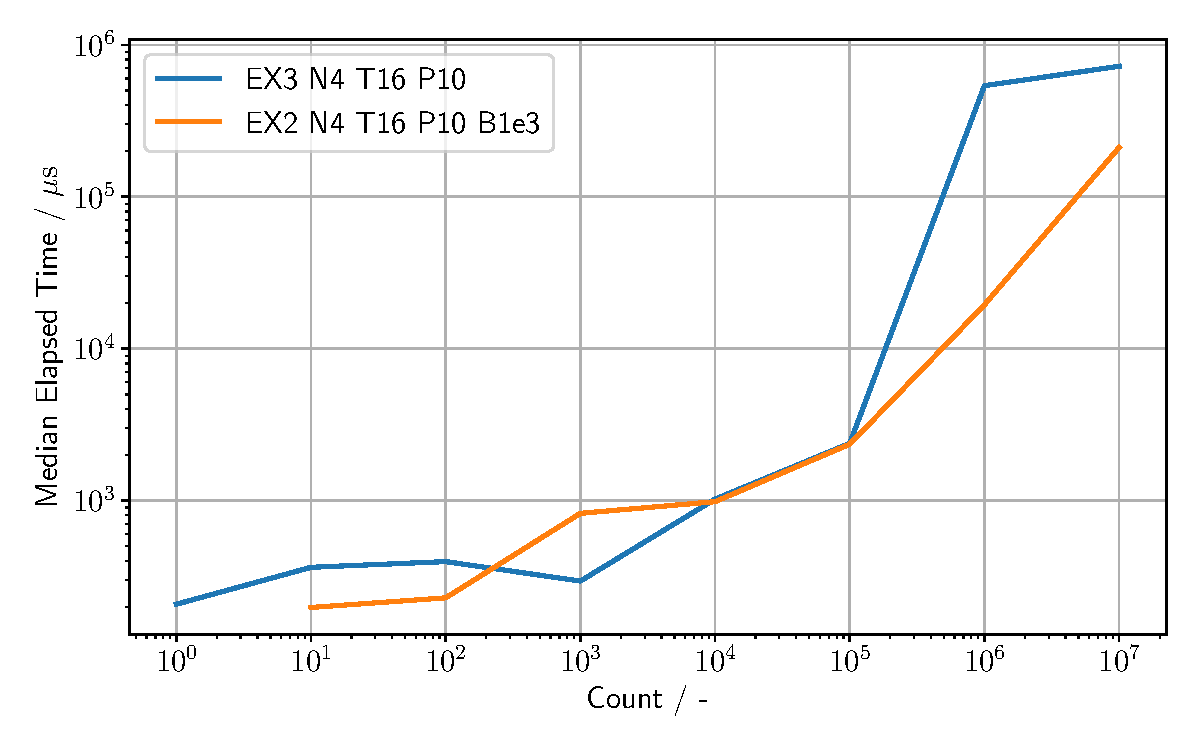
\includegraphics[width=1\linewidth]{figures/Ex3_1.pdf}
        \caption{Median of elapsed time for \fun{MY\_Allreduce\_P()}. 4 nodes, 16 processes per node, powers of 10,
         static blocksize for the EX2 timing and variable blocksize for EX3 timing. 
         20 nodes, 16 processes per node and powers of 10. Performance improvement for count $10^3$.}
        \label{Ex3_1_p}
    \end{center}
\end{figure}

\pagebreak

In figure \ref{Ex3_2_p} we show the configuration of 4 nodes, both powers and all 3 tasks per processes numbers.
It can be seen that the slope decreases again at certain numbers of counts for both powers of 2 and 10, 
this is most likely not due to the improved algorithm, but due to our variable blocksize.

\begin{figure}[h]

    \begin{center}
        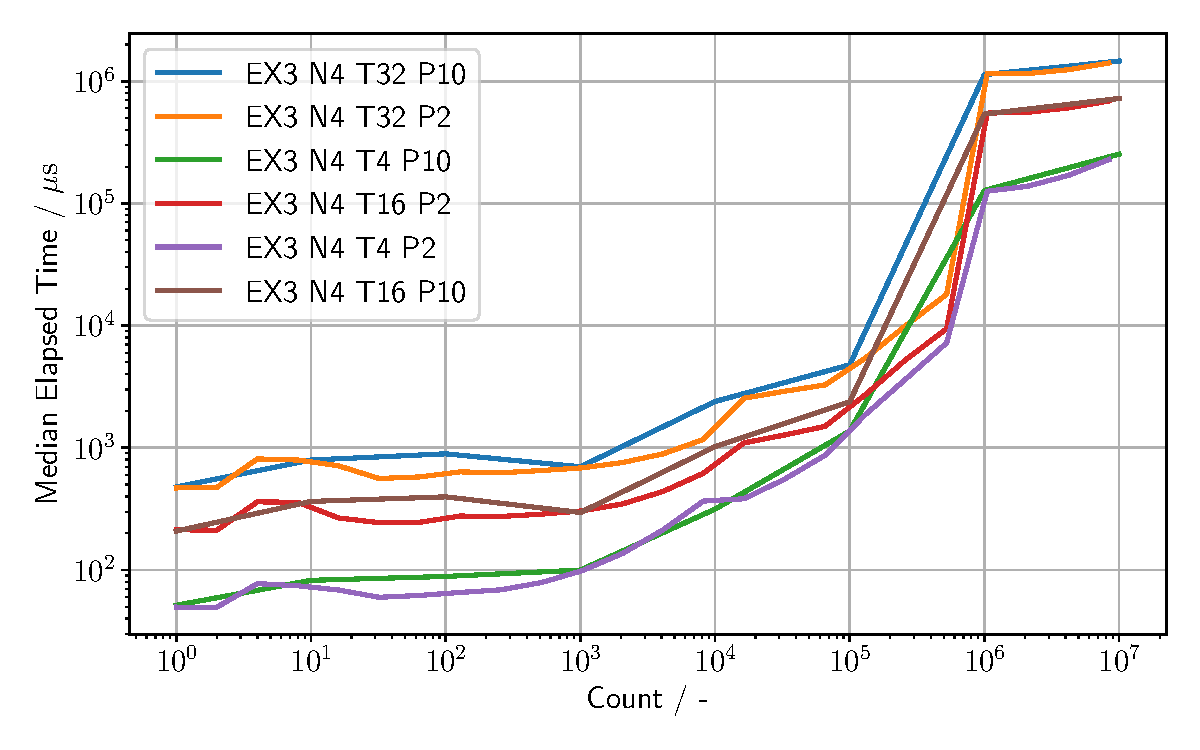
\includegraphics[width=1\linewidth]{figures/Ex3_2.pdf}
        \caption{Median of elapsed time for \fun{MY\_Allreduce\_P()}. 4 nodes, 4 processes per node, 
        powers of 2 and 10, and variable blocksize. Performance improvements visible most likely
        due to variable blocksize.}
        \label{Ex3_2_p}
    \end{center}
\end{figure}